\section{American Fuzzy Lopper (AFL)} \label{sec:2.2}

Michal Zalewski developed American Fuzzy Lopper as a coverage-guided greybox fuzzer. He introduces this open-source project as \say{a security-oriented fuzzer that employs a novel type of compile-time instrumentation and genetic algorithms to automatically discover clean, interesting test inputs that trigger new internal states of the targeted binary. This substantially improves the functional coverage for the fuzzed code. The compact synthesized corpus produced by the tool help seed other, more labor- or resource-intensive testing regimes down the road.} \cite{zalewski2014american} AFL is designed to perform \textbf{fast} and \textbf{reliable}, and at the same time, benefits from the \textbf{simplicity} and \textbf{chainability} features \cite{about_afl}:

\begin{itemize}
    \item \textbf{Speed:} Avoiding the time-consuming operations and increasing the number of executions over time.
    \item \textbf{Reliability:} AFL takes strategies that are program-agnostic, leveraging only the coverage metrics for more discoveries. This feature helps the fuzzer to perform consistently in finding the vulnerabilities in different programs.
    \item \textbf{Simplicity:} AFL provides different options, helping the users enhance the fuzz testing in a straightforward and meaningful way. 
    \item \textbf{Chainability:} AFL can test any binary which is executable and is not constrained by the target software. A driver for the target program can connect the binary to the fuzzer.
\end{itemize}

AFL uses both dynamic and static instrumentation to profile executions; the first one requires binary files, and the SI steps in at compile-time (requiring source code). AFL uses QEMU (Quick EMUlator) to perform the DI. DI allows instrumentating closed-source binaries \cite{afl_qemu}. The emulator wraps the genuine instructions into analyzable modules, which helps with the construction of the CFG. SI is a faster method for fuzzing with AFL, which causes an average slow down of 10-100\% for each execution. AFL currently uses \textbf{LLVM} (Low-Level Virtual Machine) for injecting code coverage instructions into the program \cite{afl-llvm}. Unlike DI, \texttt{llvm-mode} configures the source code such that the CPU can execute the instructions directly, and there is no need for any extra environment to profile executions. In this article, the LLVM mode is described in more detail.

\subsection{LLVM} \label{sub:2.2.1}

\say{The LLVM Project is a collection of modular and reusable compiler and toolchain technologies. Despite its name, LLVM has little to do with traditional virtual machines. The name \textbf{LLVM} itself is not an acronym; it is the full name of the project.} \cite{llvm} Two of the relevant projects used by AFL are as follow:

\begin{itemize}
    \item The \textbf{LLVM Core} libraries contain source/target-independent optimizers as well as code generators for popular CPUs. These well-documented modules assist development of a custom compiler in every step (\textit{pass}) through the conversion of source code to executable binary file.
    
    \item \textbf{Clang} \cite{clang} provides a front-end for compiling C language family (C, C++, Objective C/C++, OpenCL, CUDA, and RenderScript) for the LLVM Project. Clang uses the LLVM Core libraries to generate an \textit{Intermediate Representation} (\textbf{IR}) of the source code \cite{lattner2004llvm}. The IR is then translated into an executable binary for the machine's CPU (Figure \ref{fig:llvm}).
\end{itemize}

\begin{figure}[!b]
    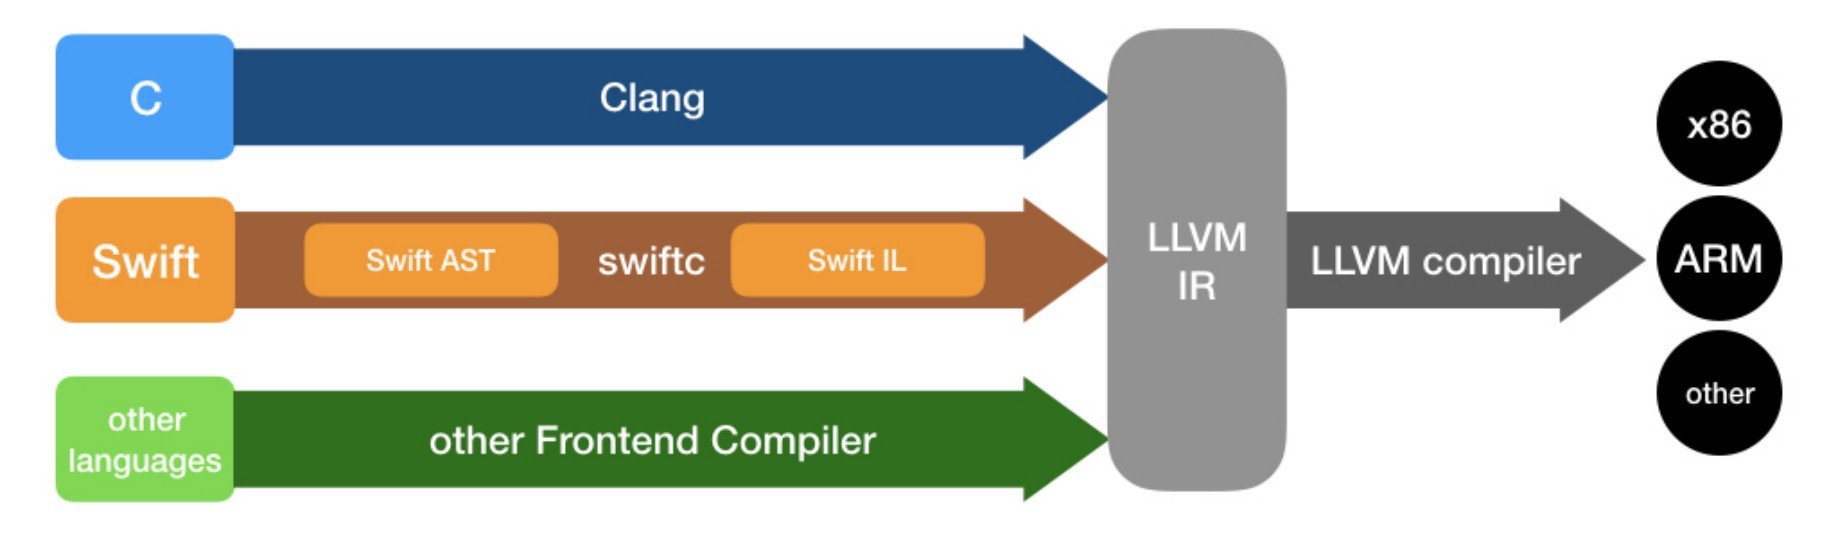
\includegraphics[width=\textwidth]{Chapter2/llvm.png}
    \centering
    \captionsetup{justification=centering}
    \caption{LLVM architecture: A front-end compiler generates the LLVM IR, and then it is converted into machine code \cite{omni_sci}}
    \label{fig:llvm}
\end{figure}

AFL utilizes the compilation \textit{passes} of Clang with a custom \textit{module pass}. Passes are the modules performing the transformations and optimizations of a compilation. A pass builds the analysis results that are used by these transformations, and a sequence of passes construct the compiler. AFL's instrumentation takes the whole program as one module and analyses it to detect the basic blocks.

\subsubsection{Static Instrumentation and Code Coverage}
\label{instrumentation}

AFL's static instrumentation starts with the allocation of a shared memory. This shared memory stands between AFL's fuzzer and each program's execution. Everytime the instrumentated program is run, the injected instructions fill the shared memory with the coverage status of the execution. After the termination of the process, AFL continues its fuzzing procedure. Shared memory is updated with new execution's data, and AFL can use it to evaluate the performance of the recent execution. The runtime initialization recipe is saved in \texttt{llvm-mode/waffle-llvm-rt.o.c} of the project.

\begin{lstlisting}[language=C++,style=CodeStyle,label={lst:hash},caption={Select element and update in shared\_mem}]
    cur_location = <COMPILE_TIME_RANDOM>;
    shared_mem[cur_location ^ prev_location]++; 
    prev_location = cur_location >> 1;
\end{lstlisting}

Next, the AFL's module pass is called. In this pass, AFL iterates over the all functions of the module, and digs into the basic blocks of the functions. Clang statically generates the CFG of the program, and AFL uses this graph to find the entry of each basic block. To store the execution path, AFL marks each basic block with a random integer. The execution path is hashed with these values as the program steps into basic blocks. This hashed number specifies an index on the shared memory. These static calculations end with an increment on the content of the hashed location. [Listing \ref{lst:hash}]
An snippet of the AFL's instrumentation pass is shown in Listing \ref{lst:afl-llvm}.

\lstinputlisting[language=C++,style=CodeStyle,label={lst:afl-llvm},caption={AFLCoverage module}]{Codes/Chapter2/afl_llvm_pass.cpp}

Figure \ref{fig:instrumentation} shows an example of how the instrumentation configures the paths. Suppose that we have an instrumented program with the random values which are set in compile time. (for simplicity, suppose that initially random value $cur\_location=1010$) Running the first basic block assigns $CUR\_HASH$ to $73\oplus1010=955$; the content of index $955$ of shared memory is then increased by one, and the execution continues to the next basic block. Supposing basic block 2 is the next block, the content of $shared\_mem[310\oplus(73>>1)=274]$ is incremented by one, and so on. After the termination of this run, the content of the shared memory contains a hashing of the path. For instance, taking the path $1\rightarrow2\rightarrow5$ results in an array of zeros except for $\{51: 1, 274: 1, 955: 1\}$ as the hashing of the path (\textit{\{index: value\}}).

\begin{figure}[htpb]
    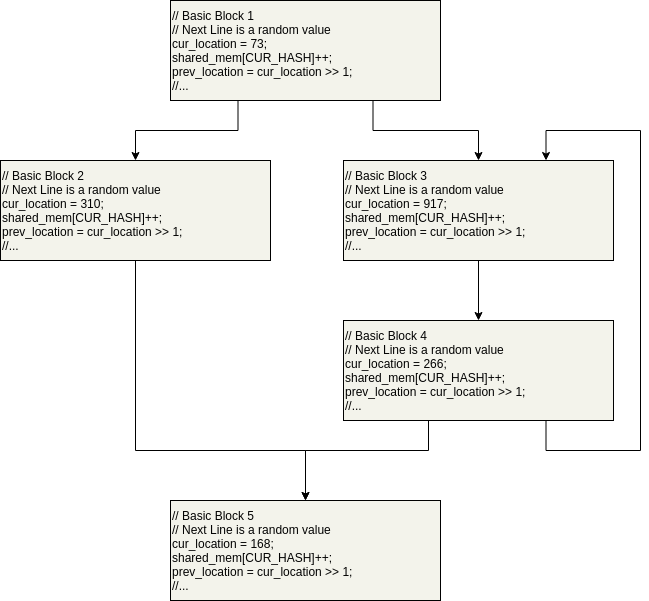
\includegraphics[width=\textwidth]{Chapter2/instrumentation.png}
    \centering
    \captionsetup{justification=centering}
    \caption{Example for instrumented basic blocks}
    \label{fig:instrumentation}
\end{figure}

\subsection{AFL Fuzz}

\textit{afl-fuzz.c} has the instructions for fuzzing the target instrumented-program. The Algorithm \ref{algo:afl} illustrates a brief pseudocode of the execution of \textit{afl-fuzz}:

% main
%     initialize the fuzzer
%     while fuzzing is not terminated:
%         cull the queue of tests and update the bitmap
%         select the first entity of the queue, as E
%         fuzz(E)

% calibrate:
%     /* Calibrate a new test case. This is done when processing the input directory
%    to warn about flaky or otherwise problematic test cases early on; and when
%    new paths are discovered to detect variable behavior and so on. */

% trimming:
%     /* Trim all new test cases to save cycles when doing deterministic checks. The
%    trimmer uses power-of-two increments somewhere between 1/16 and 1/1024 of
%    file size, to keep the stage short and sweet. */

\begin{algorithm}
    % \DontPrintSemicolon % Some LaTeX compilers require you to use \dontprintsemicolon instead
    \KwIn{\textbf{$in\_dir$}, \textbf{$out\_dir$}, $instrumented$ \textbf{$Target$}}
    initialize fuzzer\;
    \While{fuzzing is not terminated} {
      $cull\_queue()$\;
      $Entry \leftarrow q.first\_entry()$\;
      $fuzz\_one(Entry)$\;
    }
    \caption{afl-fuzz}
    \label{algo:afl}
\end{algorithm}

After the environmental initializations, the fuzzing loop continues until receiving a termination signal. In every iteration of the loop, AFL first culls the corpus of the generated entries. This method assigns a \textbf{favor-factor} (Eq \ref{eq:afl_fav_fac}) to each queue\_entry and marks the \textbf{favorite entries}, as they execute faster and the size of the files are smaller than the rest of the corpus. AFL finds a favorable path for \say{having a minimal set of paths that trigger all the bits seen in the bitmap so far, and focus on fuzzing them at the expense of the rest.} \cite{afl_git} 
\begin{equation}
    fav\_factor = e.exec\_time \times e.length
    \label{eq:afl_fav_fac}
\end{equation}

An entry is selected after culling the queue. AFL evolves the input corpus by generating new entries out of the selected input entry - \texttt{fuzz\_one()}. 

\subsubsection{fuzz\_one()}

% fuzz
%     calibrate the test case
%     trim the test cases (if needed)
%     calculate the performance score
%     bitflip
%     interesting values and dictionary usage
%     random havoc

\begin{algorithm}
    \KwIn{\textbf{$queue Entry$}}
    $test\_case \leftarrow Entry.test\_case$
    $calibrate(test\_case)$\;
    $bitflip(test\_case)$\;
    $save\_if\_interesting(test\_case)$\;
    $random\_havoc(test\_case)$\;

    \caption{$fuzz\_one$: Fuzz one Entry}
    \label{algo:fuzzone}
\end{algorithm}

Fuzzing a single entry requires the calibration of the test-cases; calibration helps AFL in evaluating the stats of the current entry. This evaluation is stored in \texttt{perf\_score}, and the number of trials for generating new inputs from the \textbf{random\_havoc} stage is calculated using the \texttt{perf\_score}. AFL, as a coverage-based fuzzer, assigns higher performance score for the entries that are executed faster and have bigger bitmaps.

The evolutionary algorithms for generating new entries are applied in two stages: \textbf{deterministic} and \textbf{random\_havoc} stages. As shown in Algorithm \ref{algo:fuzzone}, AFL initially tries the basic, deterministic algorithms. These algorithms are executed for a specific number of times, in the same order, and once for each fuzzing trial. . Bit-flipping, byte-flipping, simple arithmetic operations, using known integers and values from dictionaries, are a sequence of mutations that AFL applies on an entry in \textbf{deterministic} stage. Each one of the above operations tweak a small portion of the fuzzed input, and does not modify the file in large portions - up to 32 bits changes in each tweak.

The \textbf{havoc} stage is a cycle of stacked random tweaks. AFL assesses the current entry to insert into the queue. Each mutation is selected randomly and with a higher \texttt{perf\_score}, this stage continues more fuzzing over the current entry. The \texttt{random\_havoc} stage consists techniques such as bit flips, overwriting with random and interesting integers, block deletion, block duplication, and (if supplied) assorted dictionary-related operations \cite{afl_userguide}. An abstract implementation of the \texttt{havoc\_stage} can be found in Appendix \ref{app:havoc}.

\subsubsection{calculate\_score()}
\label{sub:calc_score}

This function calculates how much AFL desires to iterate in havoc stage, for the current entry. By default, AFL is interested in fuzzing an input with less execution-time, and simultaneously, showing more coverage, and it's generation depth is higher. The depth of a child entry is one more than the depth of it's parent. For more information, check the following abstraction of the function [Listing \ref{lst:calc_score}]: 

\lstinputlisting[language=C,style=CodeStyle,label={lst:calc_score},caption={An abstract implementation of calculate\_score()}]{Codes/Chapter2/calculate_score.c}

\subsubsection{common\_fuzz\_stuff()}
The newly fuzzed (generated) inputs must pass \texttt{common\_fuzz\_stuff()} for validating and instantiating a \texttt{queue\_entry}. The validation checks the length of the fuzzed file, executes the program and keeps the exit-value of the execution. In the end, AFL calls \texttt{save\_if\_interesting()} to insert the entry into the queue, if it is interesting. The function \texttt{has\_new\_bits()} considers how interesting an entry is.

\lstinputlisting[language=C,style=CodeStyle,label={lst:common_stuff},caption={An abstract implementation of common\_fuzz\_stuff()}]{Codes/Chapter2/common_fuzz_stuff.c}

\subsubsection{has\_new\_bits()}
AFL calls this function after each execution of the program, and the optimization of this code participates an important role.

\lstinputlisting[language=C,style=CodeStyle,label={lst:has_new_bits},caption={The implementation of has\_new\_bits()}]{Codes/Chapter2/has_new_bits.c}

\subsection{Status screen}

The \textbf{status screen} is a UI for the status of the fuzzing procedure. As it is shown in Figure \ref{fig:status_screen}, there are multiple stats provided in real-time updates:
    
\begin{figure}[!b]
    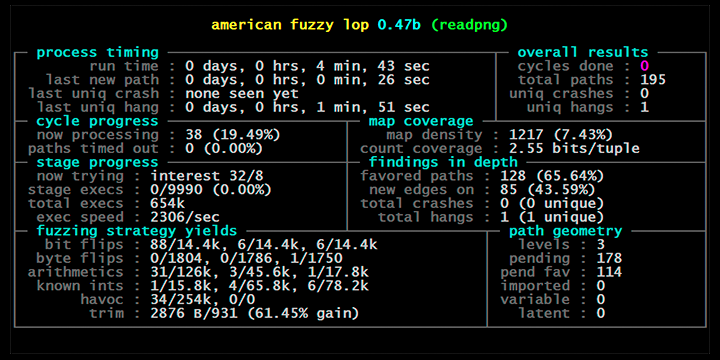
\includegraphics[width=\textwidth]{Chapter2/afl_screen.png}
    \centering
    \caption{AFL status screen}
    \label{fig:status_screen}
\end{figure} 

\begin{enumerate}
    \item \textbf{Process timing}: This section tells about how long the fuzzing process is running.
    \item \textbf{Overall results}: A simplified information about the progress of AFL in finding paths, hangs, and crashes. 
    \item \textbf{Cycle progress}: As mentioned before, AFL takes one input and repeats mutating it for a while. This section shows the information about the current cycle that the fuzzer is working on.
    \item \textbf{Map coverage}: \say{The section provides some trivia about the coverage observed by the instrumentation embedded in the target binary. The first line in the box tells you how many branches we have already hit, in proportion to how much the bitmap can hold. The number on the left describes the current input; the one on the right is the entire input corpus's value. The other line deals with the variability in tuple hit counts seen in the binary. In essence, if every taken branch is always taken a fixed number of times for all the inputs we have tried, this will read "1.00". As we manage to trigger other hit counts for every branch, the needle will start to move toward "8.00" (every bit in the 8-bit map hit) but will probably never reach that extreme. 
    
    Together, the values can help compare the coverage of several different fuzzing jobs that rely on the same instrumented binary.
    }
    \item \textbf{Stage progress}: The information about the current mutation stage is briefly provided here.
    \item \textbf{Findings in depth}: The crashes and hangs and any other findings (here we have the other information about the coverage) are presented in this section.
    \item \textbf{Fuzzing strategy yields}: To illustrate more stats about the strategies used since the beginning of fuzzing, and for comparison of those strategies, AFL keeps track of how many paths were explored, in proportion to the number of executions attempted, for each of the fuzzing strategies.
    \item \textbf{Path geometry}: The information about the inputs and their depths, which says how many generations of different paths were produced in the process. For instance, we call the seeds we provided for fuzzing the "level 1" inputs. Next, a new set of inputs is generated as "level 2", the inputs derived from "level 2" are "level 3," and so on.
\end{enumerate}

\subsection{Start Fuzz Testing}

AFL requires the instrumented binary for execution. To start the instrumentation, AFL uses \textit{afl-clang}, which is built with the coverage recipe included. The following command instruments the sample program \ref{lst:sample_vul}:

\begin{lstlisting}[language=bash,style=CommandStyle,caption=Instrument $sample\_vul$.c]
    afl-clang sample_vul.c -o sample_vul_i
\end{lstlisting}

Now AFL can run this program in \textit{afl-fuzz} with the coverage instrumentations.

\begin{lstlisting}[language=bash,style=CommandStyle,caption=Execute AFL]
  # afl-fuzz -i <in_dir> -o <out_dir> [options] -- /path/to/fuzzed/app [params]
  afl-fuzz -i in_dir -o out_dir -- ./sample_vul_i
\end{lstlisting}

The fuzzing continues until the fuzz testing is stopped using a termination signal. Pressing \textit{Ctrl+C} is a common command for this purpose. All of the recorded information are accessed through the output directory \textit{out\_dir}.